\section{Сравнение с SQLite}

\subsection{Методология сравнения}

Для сравнения LSM-решения с SQLite была разработана простая система хранения на основе SQLite. Она использует базу данных, состоящую из двух таблиц. Первая таблица называется Measurement и используется для хранения измерений. Каждое измерение представлено своим ключом, временной меткой и значением, а ключ - это первичный идентификатор объекта MeasurementMeta, который хранится во второй таблице. Этот объект хранит имя тега измерения; поэтому можно выполнять поисковые операции с фильтрацией по числовому столбцу вместо текстового столбца. В таблице измерений есть индексы как для ключевого столбца, так и для столбца временной метки.

Для следующих тестов использовалась придуманная синтетическая система. Эта система имеет 10 датчиков, которые производят данные с частотой дискретизации 1 Гц. Для тестов чтения данные для этих 10 тегов были сгенерированы для трех часов измерений. Следовательно, в базе данных SQLite содержатся 108000 записей или точек, или 10800 точек на каждый тег. Библиотека LSM также содержит 108000 записей, разделенных на 10 файлов для каждого тега, по 10800 точек в каждом. Для тестов записи данные для этих 10 тегов генерируются для различных временных диапазонов и затем сохраняются в обоих механизмах хранения.

Для тестирования обоих механизмов хранения использовался стандартный механизм тестирования Go. Он запускает целевой код несколько раз, пока тестовая функция не проработает достаточно долго, чтобы время ее выполнения можно было надежно измерить ~\cite {go_benchmark}. Этот механизм дает результат, который измеряется в ns/op, наносекундах на итерацию; для данных тестов итерация - это один вызов чтения или записи в хранилище.

Все тесты выполнялись на ПК с Intel Core i5-8400 под управлением Ubuntu 18.04, файлы данных для обоих хранилищ хранились на твердотельном накопителе NVMe.

\subsection{Чтение всего диапазона данных}

Этот тест измеряет время считывания для различных временных диапазонов, в то время как операция выполняется для полных трех часов измерений. Результаты этого теста представлены на рисунке ~\ref{fig3}. Как видно, GoLSM примерно в два раза быстрее SQLite по запросам на чтение. Стоит отметить, что уровень $C_0$ LSM-дерева не играет существенной роли в ускорении извлечения данных, поскольку временной диапазон выбирается случайным образом из всех трех часов измерений, в то время как уровень $C_0$ содержит только последние две минуты измерений.

\begin{figure}[h!]
	\centering
	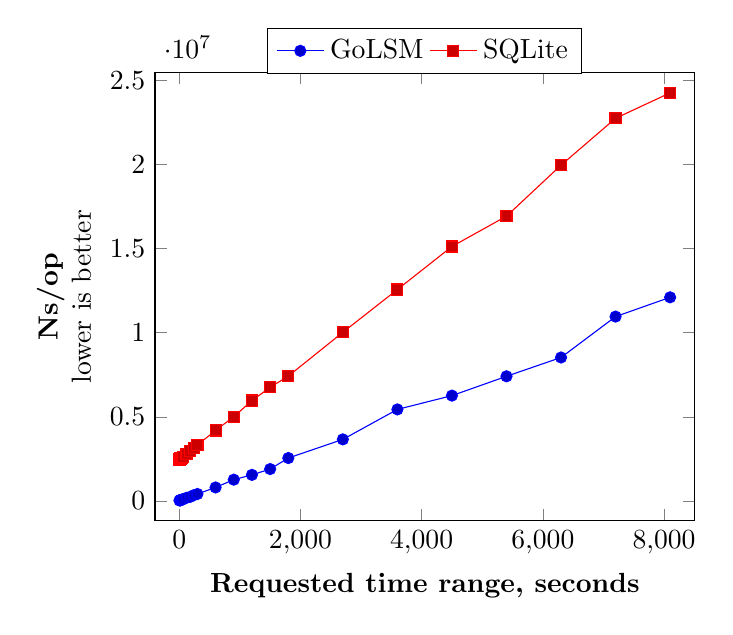
\begin{tikzpicture}
        % first provide your data as table, so later the data can
        % easily be accessed for various stuff
        \pgfplotstableread{
            x    y  z
5 29245				    2468624
10 34331			    2488443
15 41885			    2487442
20 47359			    2533488
25 51261			    2517353
30 62037			    2529031
45 76538			    2571565
60 101490			    2611909
120 185574			    2787438
180 241142			    2986666
240 341329			    3155070
300 412849			    3327132
600 801901			    4190652
900 1264738			    5008636
1200 1549898			    5966411
1500 1895210			    6753930
1800 2550300			    7420697
2700 3659991			    10027510
3600 5442224			    12570023
4500 6261830			    15128483
5400 7410561			    16932040
6300 8529041			    19965360
7200 10960360			    22752193
8100 12106688			    24262132
        }{\data}
    \begin{axis}[
        x tick style={/pgf/number format/1000 sep=},
	    ylabel style={align=center},	
	    ylabel = \textbf{Ns/op}\\lower is better,
	    xlabel style={align=center},	
	    xlabel = \textbf{Requested time range, seconds},
	    enlargelimits=0.05,
	    legend style={
	        at={(0.5,1.1)}, anchor=north,legend columns=-1
	    },
    ]
        % then your `\addplot commands change to
        \addplot table [x=x,y=y] {\data};
        \addlegendentry{GoLSM}
        \addplot table [x=x,y=z] {\data};
        \addlegendentry{SQLite}
    \end{axis}
\end{tikzpicture}
	\caption{Чтение всего диапазона данных.} \label{fig3}
\end{figure}

Как видно, хранилище LSM до 50 раз быстрее, чем SQLite в небольшом диапазоне запросов (51251 нс/операцию для GoLSM и 2517353 нс/операцию для SQLite в диапазоне 25 секунд) и до двух раз быстрее в большом диапазоне запросов (12106688 нс/оп и 24262132 нс/оп в диапазоне 2 ч 15 мин). Эта большая разница может быть вызвана использованием индекса в памяти для каждого файла SST, который работает лучше, чем индексация в SQLite. Повышение эффективности для малого диапазона запросов может быть вызвано тем фактом, что малый запрошенный диапазон с большей вероятностью умещается в пределах уровня $C_0$ дерева LSM, поэтому медленное извлечение из SST не вызывается.

\subsection{Чтение за последние три минуты}

Этот тест измеряет время считывания для различных временных диапазонов, в то время как операция выполняется для последних трех минут измерений. Результаты этого теста показаны на рисунке ~\ref{fig4}. Поскольку уровень $C_0$ LSM-дерева содержит последние две минуты измерений, более вероятно, что запрос будет соответствовать уровню $C_0$ без необходимости запрашивать данные с уровня $C_1$. Таким образом, извлечение данных в два раза быстрее, чем извлечение данных за все три часа измерений, как показано на рисунке ~\ref{fig5}. 

\begin{figure}[!htb]
	\begin{minipage}{0.48\textwidth}
		\centering
		\resizebox{\textwidth}{!}{%
			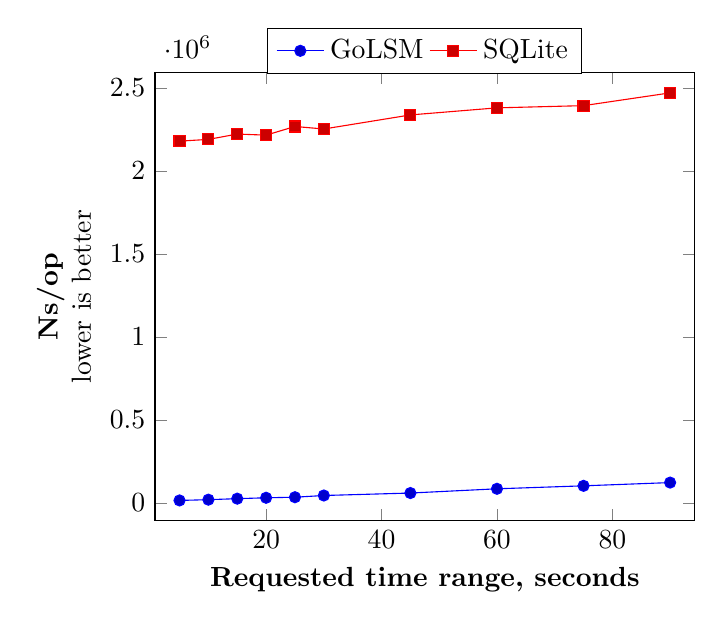
\begin{tikzpicture}
        % first provide your data as table, so later the data can
        % easily be accessed for various stuff
        \pgfplotstableread{
            x    y  z
5 14164				    2179781
10 18772			    2190392
15 24835			    2222522
20 30221			    2216021
25 33592			    2268216
30 43931			    2253056
45 58727			    2337832
60 84315			    2380516
75 102221			    2393851
90 121761			    2470748
        }{\data}
    \begin{axis}[
        x tick style={/pgf/number format/1000 sep=},
	    ylabel style={align=center},	
	    ylabel = \textbf{Ns/op}\\lower is better,
	    xlabel style={align=center},	
	    xlabel = \textbf{Requested time range, seconds},
	    enlargelimits=0.05,
	    legend style={
	        at={(0.5,1.1)}, anchor=north,legend columns=-1
	    },
    ]
        % then your `\addplot commands change to
        \addplot table [x=x,y=y] {\data};
        \addlegendentry{GoLSM}
        \addplot table [x=x,y=z] {\data};
        \addlegendentry{SQLite}
    \end{axis}
\end{tikzpicture}
		}
		\caption{Чтение всего диапазона данных}\label{fig4}
	\end{minipage}\hfill
	\begin{minipage}{0.48\textwidth}
		\centering
		\resizebox{\textwidth}{!}{%
			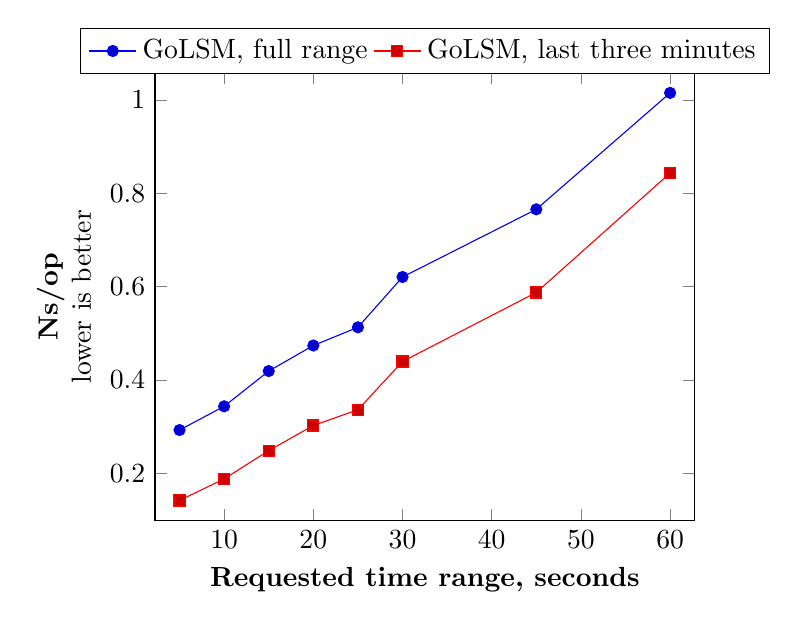
\begin{tikzpicture}
        % first provide your data as table, so later the data can
        % easily be accessed for various stuff
        \pgfplotstableread{
            x    y  z
5	29245	14164
10	34331	18772
15	41885	24835
20	47359	30221
25	51261	33592
30	62037	43931
45	76538	58727
60	101490	84315
        }{\data}
    \begin{axis}[
        x tick style={/pgf/number format/1000 sep=},
	    ylabel style={align=center},	
	    ylabel = \textbf{Ns/op}\\lower is better,
	    xlabel style={align=center},	
	    xlabel = \textbf{Requested time range, seconds},
	    enlargelimits=0.05,
	    legend style={
	        at={(0.5,1.1)}, anchor=north,legend columns=-1
	    },
    ]
        % then your `\addplot commands change to
        \addplot table [x=x,y=y] {\data};
        \addlegendentry{GoLSM, full range}
        \addplot table [x=x,y=z] {\data};
        \addlegendentry{GoLSM, last three minutes}
    \end{axis}
\end{tikzpicture}
		}
		\caption{Разница в скорости для разных интервалов.}\label{fig5}
	\end{minipage}
\end{figure}

Если в системе предполагается чтение только самых последних данных, увеличение емкости $C_0$ может значительно улучшить производительность чтения и снизить нагрузку чтения на постоянное хранилище диска.

\subsection{Запись упорядоченных данных}

Этот тест измеряет время записи для различных временных диапазонов. В то время как данные являются упорядоченными, минимальная временная метка следующего записываемого пакета данных всегда больше, чем максимальная временная метка ранее записанного пакета. Это означает, что для каждого SST-файла в GoLSM данные добавляются только в конец SST-файла без необходимости повторять сортировку SST-файла. Результаты этого теста представлены на рисунке ~\ref{fig6}.

\begin{figure}[!htb]
	\begin{minipage}{0.48\textwidth}
		\centering
		\resizebox{\textwidth}{!}{%
			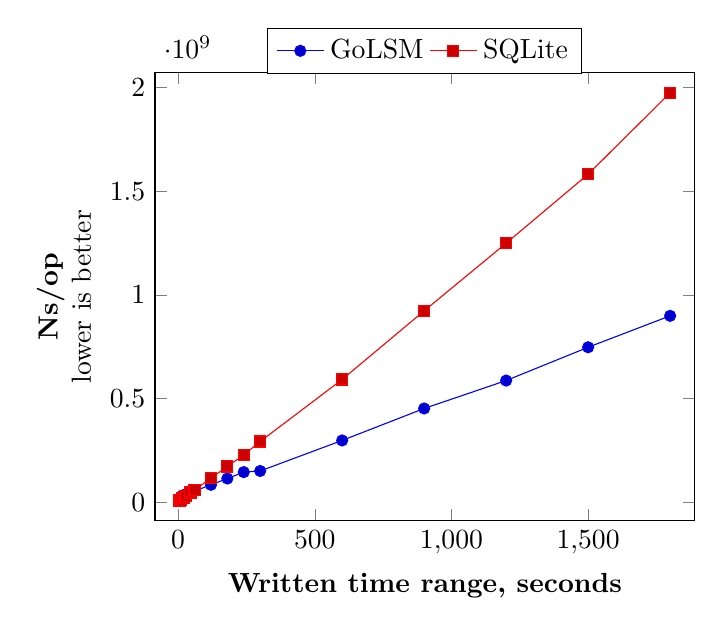
\begin{tikzpicture}
        % first provide your data as table, so later the data can
        % easily be accessed for various stuff
        \pgfplotstableread{
            x    y  z
5 15645901			    9353729
10 22956983			    11181460
15 32283634			    19307910
20 34011973			    21123025
25 33267746			    28927692
30 39930080			    30805858
45 49632256			    47978279
60 54524124			    59648520
120 84668307			    116531430
180 115137807			    173160076
240 146032654			    228964797
300 151417281			    293465746
600 298689957			    592581370
900 452684093			    923305824
1200 587385346			    1249406072
1500 747870163			    1582051745
1800 899311404			    1974174575

        }{\data}
    \begin{axis}[
        x tick style={/pgf/number format/1000 sep=},
	    ylabel style={align=center},	
	    ylabel = \textbf{Ns/op}\\lower is better,
	    xlabel style={align=center},	
	    xlabel = \textbf{Written time range, seconds},
	    enlargelimits=0.05,
	    legend style={
	        at={(0.5,1.1)}, anchor=north,legend columns=-1
	    },
    ]
        % then your `\addplot commands change to
        \addplot table [x=x,y=y] {\data};
        \addlegendentry{GoLSM}
        \addplot table [x=x,y=z] {\data};
        \addlegendentry{SQLite}
    \end{axis}
\end{tikzpicture}
		}
		\label{figure}{(а) Для большого диапазона}
	\end{minipage}\hfill
	\begin{minipage}{0.48\textwidth}
		\centering
		\resizebox{\textwidth}{!}{%
			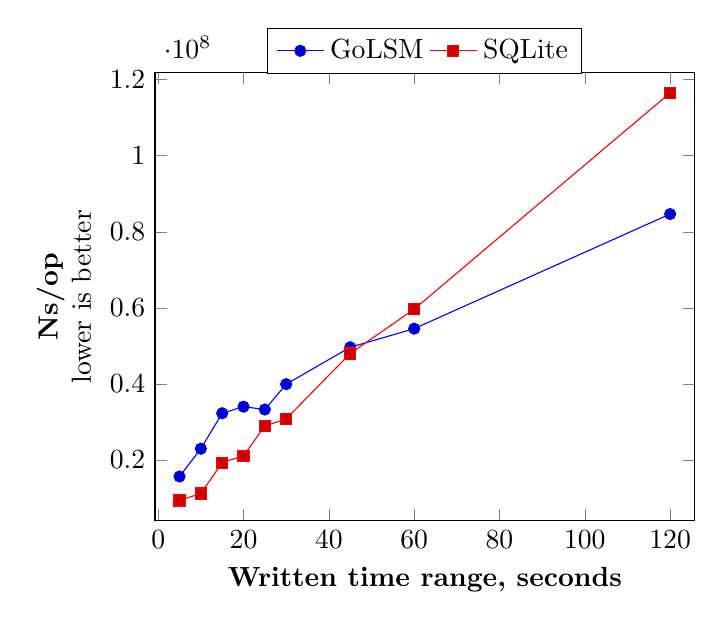
\begin{tikzpicture}
        % first provide your data as table, so later the data can
        % easily be accessed for various stuff
        \pgfplotstableread{
            x    y  z
5 15645901			    9353729
10 22956983			    11181460
15 32283634			    19307910
20 34011973			    21123025
25 33267746			    28927692
30 39930080			    30805858
45 49632256			    47978279
60 54524124			    59648520
120 84668307			    116531430

        }{\data}
    \begin{axis}[
        x tick style={/pgf/number format/1000 sep=},
	    ylabel style={align=center},	
	    ylabel = \textbf{Ns/op}\\lower is better,
	    xlabel style={align=center},	
	    xlabel = \textbf{Written time range, seconds},
	    enlargelimits=0.05,
	    legend style={
	        at={(0.5,1.1)}, anchor=north,legend columns=-1
	    },
    ]
        % then your `\addplot commands change to
        \addplot table [x=x,y=y] {\data};
        \addlegendentry{GoLSM}
        \addplot table [x=x,y=z] {\data};
        \addlegendentry{SQLite}
    \end{axis}
\end{tikzpicture}
		}
		\label{figure}{(б) Для маленького диапазона}
	\end{minipage}
	
	\caption{Запись упорядоченных данных.}\label{fig6}
\end{figure}

На рисунке ~\ref{fig6}, (а) видно, что GoLSM записывает данные в два раза быстрее, чем SQLite, в течение большого записываемого диапазона времени. Однако на рисунке ~\ref{fig6}, (б) для небольшого временного диапазона GoLSM на самом деле медленнее. Причина этого в том, что для LSM измерялось время до момента фактической записи данных в журнал фиксации, а не непосредственно в файлы SST; и когда количество записей в журнале фиксации достигает определенного порога, оно должно быть передано в SST, что вызывает скачки времени записи. Однако для записываемых больших временных диапазонов эти накладные расходы не важны по сравнению с обычно медленными пакетными вставками в SQLite.

Стоит отметить, что для вставки в SQLite необходимо составить оператор SQL Insert, который включает преобразование значения типа double в строку. Эта операция выполняется очень медленно для больших пакетов вставок (пакет из 10 тегов за 30 минут составляет 18000 точек), и использование ORM, такого как GORM, не улучшает ситуацию.

\subsection{Запись неупорядоченных данных}

Этот тест измеряет время записи для различных временных диапазонов, но, поскольку данные являются неупорядоченными, нет никаких гарантий, что все временные метки следующего пакета больше, чем временные метки ранее записанного пакета. Таким образом, пакеты могут быть получены до или после друг друга с точки зрения их временных меток. Это означает, что каждый раз, когда данные передаются из файла журнала фиксации в файлы SST, библиотека должен пересортировать весь файл SST, замедляя процесс записи. Результаты этого теста представлены на рисунке ~\ref{fig7}. Сравнение записи данных в LSM, когда данные являются упорядоченными или неупорядоченными, доступно на рисунке ~\ref {fig8}.

\begin{figure}[!htb]
	\begin{minipage}{0.48\textwidth}
		\centering
		\resizebox{\textwidth}{!}{%
			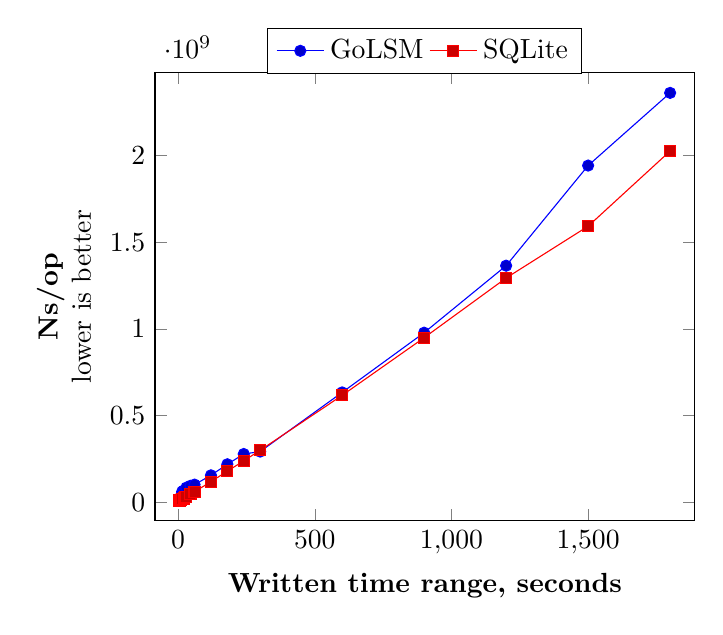
\begin{tikzpicture}
        % first provide your data as table, so later the data can
        % easily be accessed for various stuff
        \pgfplotstableread{
            x    y  z
5 20066750			    9514015
10 34790230			    10956443
15 61277403			    19290607
20 66074549			    20865090
25 63925416			    28999975
30 83572878			    30478476
45 94080339			    48656675
60 100926498			    59882936
120 154617448			    117794298
180 218391345			    178663220
240 277609792			    238031796
300 291599762			    299054072
600 633156270			    616109936
900 977887157			    948873690
1200 1364639379			    1293479495
1500 1942545058			    1592474416
1800 2362087783			    2026594877


        }{\data}
    \begin{axis}[
        x tick style={/pgf/number format/1000 sep=},
	    ylabel style={align=center},	
	    ylabel = \textbf{Ns/op}\\lower is better,
	    xlabel style={align=center},	
	    xlabel = \textbf{Written time range, seconds},
	    enlargelimits=0.05,
	    legend style={
	        at={(0.5,1.1)}, anchor=north,legend columns=-1
	    },
    ]
        % then your `\addplot commands change to
        \addplot table [x=x,y=y] {\data};
        \addlegendentry{GoLSM}
        \addplot table [x=x,y=z] {\data};
        \addlegendentry{SQLite}
    \end{axis}
\end{tikzpicture}
		}
		\caption{Запись неупорядоченных данных.}\label{fig7}
	\end{minipage}\hfill
	\begin{minipage}{0.48\textwidth}
		\centering
		\resizebox{\textwidth}{!}{%
			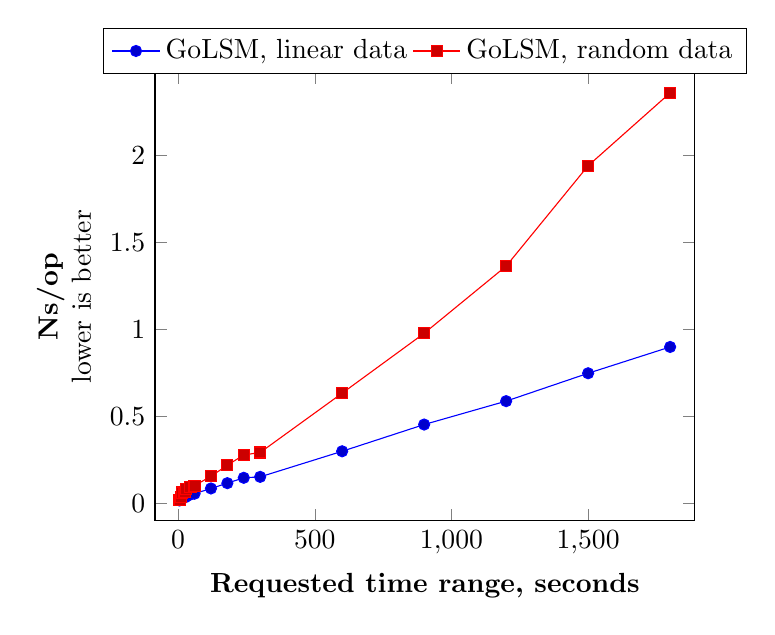
\begin{tikzpicture}
        % first provide your data as table, so later the data can
        % easily be accessed for various stuff
        \pgfplotstableread{
            x    y  z
5	15645901	20066750
10	22956983	34790230
15	32283634	61277403
20	34011973	66074549
25	33267746	63925416
30	39930080	83572878
45	49632256	94080339
60	54524124	100926498
120	84668307	154617448
180	115137807	218391345
240	146032654	277609792
300	151417281	291599762
600	298689957	633156270
900	452684093	977887157
1200	587385346	1364639379
1500	747870163	1942545058
1800	899311404	2362087783

        }{\data}
    \begin{axis}[
        x tick style={/pgf/number format/1000 sep=},
	    ylabel style={align=center},	
	    ylabel = \textbf{Ns/op}\\lower is better,
	    xlabel style={align=center},	
	    xlabel = \textbf{Requested time range, seconds},
	    enlargelimits=0.05,
	    legend style={
	        at={(0.5,1.1)}, anchor=north,legend columns=-1
	    },
    ]
        % then your `\addplot commands change to
        \addplot table [x=x,y=y] {\data};
        \addlegendentry{GoLSM, linear data}
        \addplot table [x=x,y=z] {\data};
        \addlegendentry{GoLSM, random data}
    \end{axis}
\end{tikzpicture}
		}
		\caption{Разница во времени при записи упорядоченных и неупорядоченных данных.}\label{fig8}
	\end{minipage}
\end{figure}

Как видно на рисунке ~\ref {fig7}, накладные расходы на пересортирование файлов SST при каждой записи данных настолько велики, что они занимают больше времени, чем медленные пакетные вставки в SQLite. Сравнение записи данных с этими накладными расходами с записью данных без накладных расходов показано на рисунке ~\ref{fig8}. Когда временные метки данных всегда линейно увеличиваются, это показывает, что вставки почти в три раза медленнее при записи в большом временном диапазоне (747870163 нс/операцию, или 747 мс, для записи 25 минут линейных данных и 1942545058 нс/операцию, или 1942 мс, для записи 25 минут случайных данных).